% $Header: /Users/joseph/Documents/LaTeX/beamer/solutions/conference-talks/conference-ornate-20min.en.tex,v 90e850259b8b 2007/01/28 20:48:30 tantau $
\RequirePackage{filecontents}
\begin{filecontents*}{seminar.bib}
@book{test,
author={John Smith},
title={A book},
publisher={Puplisher},
year={1742},
}
\end{filecontents*}
\documentclass{beamer}
\usepackage{graphicx}

\usepackage{latexsym}		% to get LASY symbols
\usepackage{epsfig}		% to insert PostScript figures
\usepackage{rotating}		% for sideways tables/figures
\usepackage{eufrak}
\usepackage{natbib}
\def\newblock{\hskip .11em plus .33em minus .07em}

% This file is a solution template for:

% - Talk at a conference/colloquium.
% - Talk length is about 20min.
% - Style is ornate.



% Copyright 2004 by Till Tantau <tantau@users.sourceforge.net>.
%
% In principle, this file can be redistributed and/or modified under
% the terms of the GNU Public License, version 2.
%
% However, this file is supposed to be a template to be modified
% for your own needs. For this reason, if you use this file as a
% template and not specifically distribute it as part of a another
% package/program, I grant the extra permission to freely copy and
% modify this file as you see fit and even to delete this copyright
% notice. 


\mode<presentation>
{
  \usetheme{Madrid}
  % or ...

  \setbeamercovered{transparent}
  % or whatever (possibly just delete it)
}


\usepackage[english]{babel}
% or whatever

\usepackage[latin1]{inputenc}
% or whatever

\usepackage{times}
\usepackage[T1]{fontenc}
% Or whatever. Note that the encoding and the font should match. If T1
% does not look nice, try deleting the line with the fontenc.


\title[Energy Depletion Attacks on Wireless Sensor Networks : A Survey] % (optional, use only with long paper titles)
{Energy Depletion Attacks on Wireless Sensor Networks : A Survey}
%
%\subtitle
%{Include Only If Paper Has a Subtitle}

\author[FARZANA.T] % (optional, use only with lots of authors)
{FARZANA.T}
% - Give the names in the same order as the appear in the paper.
% - Use the \inst{?} command only if the authors have different
%   affiliation.

\institute[MES College of Engineering] % (optional, but mostly needed)
{
 
  12MCS1004\\
  Computer Science \& Engineering\\
  Guide: Mrs.Aswathy babu}
% - Use the \inst command only if there are several affiliations.
% - Keep it simple, no one is interested in your street address.

%\date[CFP 2003] % (optional, should be abbreviation of conference name)
%{Conference on Fabulous Presentations, 2003}
% - Either use conference name or its abbreviation.
% - Not really informative to the audience, more for people (including
%   yourself) who are reading the slides online

\subject{Theoretical Computer Science}
% the beginning of each subsection:
\AtBeginSubsection[]
{
  \begin{frame}<beamer>{Outline}
    \tableofcontents[currentsection,currentsubsection]
  \end{frame}
}


% If you wish to uncover everything in a step-wise fashion, uncomment
% the following command: 

%\beamerdefaultoverlayspecification{<+->}


\begin{document}

\begin{frame}
  \titlepage
\end{frame}

%\begin{frame}{Outline}
 % \tableofcontents
  % You might wish to add the option [pausesections]
%\end{frame}


% Structuring a talk is a difficult task and the following structure
% may not be suitable. Here are some rules that apply for this
% solution: 

% - Exactly two or three sections (other than the summary).
% - At *most* three subsections per section.
% - Talk about 30s to 2min per frame. So there should be between about
%   15 and 30 frames, all told.

% - A conference audience is likely to know very little of what you
%   are going to talk about. So *simplify*!
% - In a 20min talk, getting the main ideas across is hard
%   enough. Leave out details, even if it means being less precise than
%   you think necessary.
% - If you omit details that are vital to the proof/implementation,
%   just say so once. Everybody will be happy with that.

\subsection{Objective}
\begin{frame}{Objective}
   \begin{itemize}
   To perform a literature survey on various energy depletion attacks affected in wireless sensor networks.

   \end{itemize}
 \end{frame}  

\subsection{Introduction}
\begin{frame}{Wireless Sensor Network}
   \begin{itemize}
  \item Consists of a number of sensors spread across a geographical area. 
  \item Each sensor has wireless communication capability 
   \item Has some level of intelligence for signal processing and networking of the data
   \end{itemize}
 \end{frame} 
 

\begin{frame}{Wireless Sensor Network cntd....}  
   \begin{itemize}
  \item Sensor node has restricted power supplies, low bandwidth, small memory and limited energy. 
  \item Leads to very demanding environment to provide security. 
   \end{itemize}
 \end{frame} 

\begin{frame}{Energy Depletion Attack}
 \begin{itemize}
  \item Attacker would send data to drain a node battery and reduce network bandwidth.  
   \end{itemize}
 \end{frame} 

\subsection{Literature survey}
\begin{frame}{Literature survey}
 \begin{itemize}
  \item Wireless Sensor Network Denial of Sleep attack[1]
  \item Intrusion Tolerant routing in Wireless Sensor Network[2]
  \item Cross-Layer Design for Energy Conservation in Wireless Sensor Network[3]
   \item Energy Efficient Opportunistic Routing in Wireless Sensor Network[4] 
   \item Sleep Deprivation Attack Detection in  Wireless Sensor Network[5]
   \item Vampire Attack: Draining Life from  Wireless Sensor Network[6]
   \end{itemize}
 \end{frame} 
 
 
\subsection{Wireless Sensor Network Denial of Sleep attack[1]}
\begin{frame}{Wireless Sensor Network Denial of Sleep attack[1]}
\begin{itemize}
\item A subset of the denial of service class of network attacks targets on MAC layer.
\item Penetrates a device's power management system to reduce the opportunities to transition into lower power states.
\item Analyses energy resource vulnerabilities at MAC level.
\item Avoided by the introduction of G-MAC protocol.
\end{itemize}
\end{frame}


\begin{frame}{Wireless Sensor Network Denial of Sleep attack[1]}
\begin{itemize}
\item G-MAC - Gateway MAC protocol.
\item Energy efficient sensor MAC protocol designed to coordinate transmissions within a cluster.
\item G-MAC periodically elects a new gateway node to equally distribute the energy requirements among all of sensors.
\item Cluster nodes only respond to the gateway node.
\item Network attackers cannot penetrate link layer of G-MAC protocol.
\end{itemize}
\end{frame}

\begin{frame}{Wireless Sensor Network Denial of Sleep attack[1]}
\begin{itemize}
\item Advantage

Perform well in all traffic situations.
\item  Disadvantage 

All cluster nodes are dependent on gateway node.

Deals only with MAC layer depletion attack.
\end{itemize}
\end{frame}

\subsection{Intrusion Tolerant routing in Wireless Sensor Network[2] }
\begin{frame}{Intrusion Tolerant routing in Wireless Sensor Network[2]}
\begin{itemize}
\item Main objective is that design of intrusion tolerant secure WSN.
\item Single compromised node can disrupt only a localised portion of the network.
\item Introduces a new protocol INSENS to achieve intrusion tolerance.
\item INSENS : INtrusion-tolerant routing protocol for wireless SEnsor NetworkS.
\end{itemize}
\end{frame}


\begin{frame}{Intrusion Tolerant routing in Wireless Sensor Network[2] cntd....}
\begin{itemize}
\item INSENS construct a forwarding table at each node to communicate between sensor node and base station.
\item Multipath routing is built to achieve secure routing.
\item Symmetric key cryptography is used for authentication between base station and sensor node.
\item Limits flooding of messages by allowing communication only between base station and sensor node.
\end{itemize}
\end{frame}

\begin{frame}{Intrusion Tolerant routing in Wireless Sensor Network[2] cntd....}
\begin{itemize}
\item Advantage

Minimize communication and computation overhead at sensor nodes.

\item Disadvantage

Maximize communication and computation overhead at base station.
\end{itemize}
\end{frame}


\subsection{Cross-Layer Design for Energy Conservation in Wireless Sensor Network[3]}
\begin{frame}{Cross-Layer Design for Energy Conservation in Wireless Sensor Network[3]}
\begin{itemize}
\item Considers Routing layer and MAC layer jointly.
\item Network layer:

 Sending the traffic generated by sensor node through multiple paths instead of forwarding always through same path.

\item MAC layer:

 Adjust retry limit of retransmission over each wireless link - different limits for different links.

\end{itemize}
\end{frame}

\begin{frame}{Cross-Layer Design for Energy Conservation in Wireless Sensor Network[3] cntd...}
\begin{itemize}
\item Advantage 

Reduces energy consumption.
\item Disadvantage

Does not consider any attack.
\end{itemize}
\end{frame}

\subsection{Energy Efficient Opportunistic Routing in Wireless Sensor Network[4]}
\begin{frame}{Energy Efficient Opportunistic Routing in Wireless Sensor Network[4]}
\begin{itemize}
\item Opportunistic routing is based on broadcast transmission of data packets.
\item Receptors need to be coordinated in order to avoid duplicated transmission.
\item Achieved by ordering the forwarding node according to some criteria.
\item Here nodes in the forwarder list are prioritized.
\item Lower priority forwarder will discard the packet if packet has been forwarded by a higher priority forwarder.
\end{itemize}
\end{frame}

\begin{frame}{Energy Efficient Opportunistic Routing in Wireless Sensor Network[4] cntd.....}
\begin{itemize}
\item Advantage

Concentrates on selecting and prioritizing the forwarder list to  minimize the total energy of network.
\item Disadvantage

Does not consider any attack at routing level.
\end{itemize}
\end{frame}


\subsection{Sleep Deprivation Attack Detection in  Wireless Sensor Network[5]}
\begin{frame}{Sleep Deprivation Attack Detection in  Wireless Sensor Network[5]}
\begin{itemize}
\item Attack prevents the nodes from going in to sleep mode.
\item Results depleting the battery and reducing the sensor lifetime from years to days.
\item Proposes a hierarchical model to detect sensor nodes affected by this attack.
\item Uses cluster based mechanism.
\end{itemize}
\end{frame}

\begin{frame}{Sleep Deprivation Attack Detection in  Wireless Sensor Network[5] cntd...}
\begin{itemize}

\item Depending on battery capacity,sensor nodes are categorised as:


\item Sink gateway
\item Cluster-in-charge
\item Sector monitor
\item Sector-in-charge
\item Leaf node

\end{itemize}
\end{frame}


  
  \begin{frame}{Sleep Deprivation Attack Detection in  Wireless Sensor Network[5] cntd...}
\begin{itemize}
\item Advantage

Increases energy efficiency
\item Disadvantage

High communication overhead in some cases
\end{itemize}
  
  \end{frame}
  
  
\subsection{Vampire Attack: Draining Life from  Wireless Sensor Network[6]}
\begin{frame}{Vampire Attack: Draining Life from  Wireless Sensor Network[6]}
\begin{itemize}
\item Composition and transmission of a message that causes more energy to be consumed by the network.
\item Resource depletion attacks at the routing protocol layer, which permanently disable networks by quickly draining node's battery power.
\item All protocols are susceptible to Vampire attacks.
\item  Do not disrupt immediate availability, but rather work over time to entirely disable a network.
\end{itemize}
\end{frame}

\begin{frame}{Vampire Attack: Draining Life from  Wireless Sensor Network[6] cntd....}
\begin{itemize}
\item Employs vampire attack on existing routing protocol PLGP during packet transmission phase.

\item PLGPa is proposed to avoid vampire attack.
\end{itemize}
\end{frame}

\begin{frame}{Vampire Attack: Draining Life from  Wireless Sensor Network[6] cntd....}
\textbf{Advantage}:
\begin{itemize}
 

\item Vampire attack identified and can increase the networks life time.
\end{itemize}
 \textbf{Disadvantage:}
\begin{itemize}
 
\item Only packet transmission phase is avoided from vampire attack, route discovery phase is not considered.

\item Only  PLGP is considred,how the proposed solution works in other routing protocol is not considered.
\end{itemize}
\end{frame}

 \begin{frame}{Comparison}
  \begin{figure}[hbtp]
  \center
  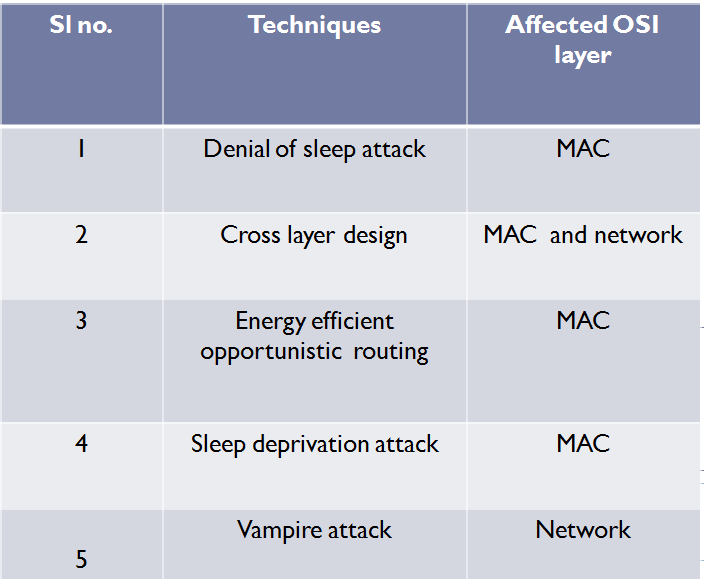
\includegraphics[scale=0.5]{tab.png}
  \caption{Comparison table} 
  \end{figure}
 \end{frame}

 \subsection{Conclusion}
\begin{frame}{Conclusion}
Performed a literature survey on various energy depletion attacks in WSN.
\end{frame}

 \subsection{References}
\begin{frame}
\frametitle{References}
\footnotesize{
\begin{thebibliography}{99}



\bibitem[Label1, 2011]{key1}[1] Michael Brownfield,Yatharth Gupta,
 \newblock "Wireless Sensor Network Denial of Sleep Attack",
 \newblock \emph{Proceedings of 2005 IEEE workshop on information assurance,June 2005}.

 
  \bibitem[Label1, 2011]{key2}[2] Jing Deng, Richard Han, Shivakanth mishra,
 \newblock "INSENS: Intrusion-Tolerant routing in Wireless Sensor Networks",
 \newblock \emph{University of Colorado,Department of computer science Technical report,June 2006 }.

\bibitem[Label1, 2011]{key3}[3] Fatma Bouabdullah, Nizar Bouabdullah,Raouf Bouabdullah 
 \newblock "Cross-layer Design for Energy Conservation in  Wireless Sensor Networks",
 \newblock \emph{IEEE GLOBECOM 2008,New Orleans,USA,December 2008}.
 \bibitem[Label1, 2011]{key4}[4] Xufei Mao,Shaojie Tang, Xiahua Xu,
 \newblock "Energy efficient Oppurtunistic Routing in Wireless Sensor Network
s",
 \newblock \emph{IEEE transactions on parellel and distributed systems, VOL. 12, NO. 2, February 2011 }

\bibitem[Label1, 2011]{key5}[5] Tapaliana Bhattasali,Rituparna Chaki,Sugata Sanyal
 \newblock "Sleep Deprivation Attack Detection in Wireless Sensor Networks",
 \newblock \emph{International journal of computer applications(0975-8887)vol 40- No: 15,February 2012 }
 
 \bibitem[Label1, 2011]{key6}[6] Eugene Y. Vasserman, Nicholas Hopper,
 \newblock " Vampire Attacks: Draining Life from Wireless Ad Hoc Sensor Networks",
 \newblock \emph{IEEE transactions on mobile computing, VOL. 12, NO. 2, February 2013 }
 
  \bibitem[Label1, 2011]{key7}[7] Yazeed Al-Obaisat,Robin Braun,
 \newblock "On Wireless Sensor Networks: Architectures,Protocols,Applications and Management",
 \newblock \emph{Institute of Information and Communication Technologies,May 2004 }
  
\end{thebibliography}
}
\end{frame}

 
\begin{frame}
\centerline{Thank You}
\end{frame}
% End of slides

\end{document}

